\documentclass[10pt]{article}
\usepackage{amsmath}
\usepackage{amsfonts}
\usepackage{ulem}
\usepackage{multirow}
\usepackage{pdfpages}
\usepackage{tabto}
\usepackage{fancyvrb}
\usepackage{listings}
\usepackage{url}
\usepackage{graphicx}
\usepackage{listing}
%used to set margins
\usepackage[margin=0.5in]{geometry}
\setboolean{@twoside}{false}


\title{Introduction to Robotics\\ Homework\#7}
\date{11/9/2017}
\author{Logan Lembke, Donovan Torgerson, Benjamin Garcia}

\begin{document}
\maketitle
\newpage

\section*{1.) Write a ROS-STDR based node to direct a differential drive robot through a sequence of points. Use p-control on heading to direct the robot.}
\lstinputlisting[language=Python]{ddpid.py}
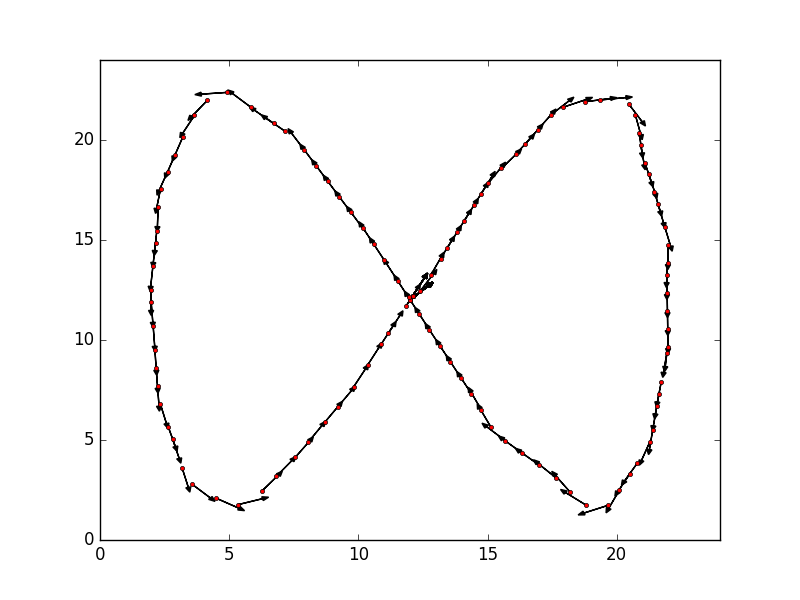
\includegraphics[width = \linewidth, height = 300px]{ddFig8.png}
\newpage
\section*{2.) Adapt your ROS-STDR program above to direct a traditional four wheel Mechanum robot.}
\lstinputlisting[language=Python]{mecpid.py}
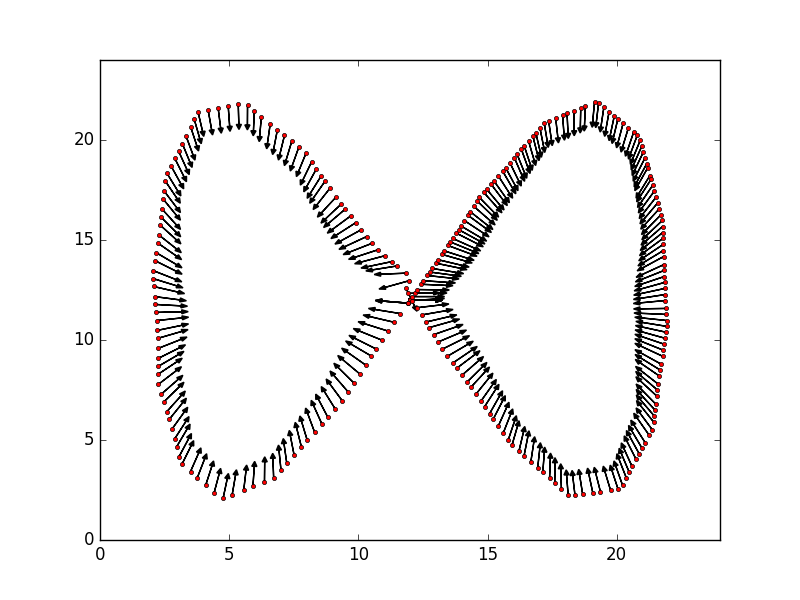
\includegraphics[width = \linewidth, height = 300px]{mecFig8.png}
\newpage
\section*{Appendix}
\subsection*{Additional Modules}
\lstinputlisting[language=Python]{ddlib.py}
\newpage
\lstinputlisting[language=Python]{graph.py}
\end{document}